\documentclass[]{report}   % list options between brackets
%\usepackage{showframe}% http://ctan.org/pkg/showframe
\usepackage{etoolbox}% http://ctan.org/pkg/etoolbox\makeatletter
\usepackage{varwidth}
%\patchcmd{\@makechapterhead}{\vspace*{50\p@}}{}{}{}% Removes space above \chapter head
%\patchcmd{\@makeschapterhead}{\vspace*{50\p@}}{}{}{}% Removes space above \chapter* head
\usepackage{titlesec}
\usepackage{graphicx}
\usepackage[latin1]{inputenc}
\usepackage{tgcursor}
\usepackage{hyperref}
\usepackage{tikz}
\usepackage{listings}
\usetikzlibrary{shapes,arrows}
\usetikzlibrary{automata,positioning}
\titleformat{\chapter}[display]   
{\normalfont\huge\bfseries}{\chaptertitlename\ \thechapter}{20pt}{\Huge}   
\titlespacing*{\chapter}{0pt}{-50pt}{40pt}
\makeatother

% type user-defined commands here
\tikzstyle{decision} = [diamond, draw, fill=blue!20, text width=4.5em, text badly centered, node distance=3cm, inner sep=0pt]
\tikzstyle{block} = [rectangle, draw, fill=blue!20, text centered, rounded corners, minimum height=4em]
\tikzstyle{line} = [draw, -latex']
\tikzstyle{cloud} = [draw, ellipse,fill=red!20, node distance=3cm, minimum height=5em]

\lstset{basicstyle=\ttfamily\scriptsize}

\begin{document}

		

        \title{Construction of a Mobile Reconnaissance Robot}   % type title between braces
        \author{Derek Sewell}         % type author(s) between braces
        \date{\today}    % type date between braces
        \maketitle
		
		


		\chapter{Project Brief}             % chapter 1
			\section{Background Information}     % section 1.1
				Robots are seeing an increased use in today's
				society. They are used in a variety of different areas, ranging from household cleaning
				(such as the Roomba\footnote{An automated vacuum - http://www.irobot.com/us/learn/home/roomba.aspx})
				to national defence. With the advent of cheaper and more accessible consumer electronics it has never been
				easier to construct your own robot. Using newly released electronics designed to make building things such
				as robots easier, I shall attempt to construct my own functioning robot and document this process.
			
			\section{Project Proposal}
				The first step was to decide what type of robot to make. The word \emph{robot} is fairly ambiguous and thus
				it is difficult to sort it into different sub sections. \emph{Robot}\ is defined as
				\emph{a machine capable of carrying out a complex set of instructions automatically} \cite{robotdef}.
				This discounts remote control vehicles from being robots as they are not autonomous, so in order for my 
				creation to be counted as a robot it must have at least some level of autonomy.
					
				Since this is my first attempt at a project of this scale, I think it best that the robot should be kept
				simple yet functional. To achieve this I shall create small size box vehicle which operates remotely. This
				keeps the components of the robot inexpensive whilst providing enough service for the robot to be
				considered useful and thus worth creating.
				
				Although the vehicle described is not technically a robot I shall aim to add some degree of automation at
				a later stage once the "robot" has been built. This is so that I can have an idea of the abilities and
				functions of my construction and can create an automation program which complements the strengths of my 
				robot so as to perform a useful task.

					
				\subsection{Purpose}
					The main purpose of the robot other than proof of concept shall be for reconnaissance. Using cellular
					networks (more on that in the research section) the range that the robot could travel would only influenced by
					the battery life, availability of mobile phone signal and terrain. This enables the robot to be a vessel of
					exploration for the surrounding area. It could also be used to explore areas with dangerous hazards, so that
					human life is not risked in the process. However in practice I do not have access to such environments so this
					is a theoretical use of the robot only.
		
		\chapter{Research}
			\section{Computing platform}
				In order to transmit footage to the user, the robot will need to be equipped with a camera. The cheapest type of camera
				available for purchase would be a webcam. A webcam is typically used for visual contact whilst talking over
				VoIP\footnote{Voice over Internet Protocol - Talking to people through the internet instead of on the phone, used in
					applications such as Skype}.
				Because of their limited functions webcams contain very little equipment apart from the camera. They have no storage mechanisms
				and typically no way to transmit their video other than through USB. In order to use these webcams I will need a computing
				platform which supports webcams and has the ability to connect to the internet.
				
				The perfect platform for the job would be the Raspberry Pi (Referenced sometimes as just Pi). Released on the 29 February 2012 the Raspberry Pi sold out in about
				15 minutes, amassing over two million expressions of interest or pre-orders\cite{rasporder}. The reason for such high demand is that
				the Raspberry Pi is small, lightweight and cheap, qualities that are very rarely seen in any other computer and these are the qualities
				which I will need for my robot. The orders have died down since then
				and I was able to purchase one for the robot. The Raspberry Pi is essentially a credit card sized computer capable of performing
				many of the functions a much larger and more expensive desktop computer can. These functions include interfacing with a webcam and
				transmitting and receiving data via the internet. The Raspberry Pi was designed to run on Linux and the particular flavour of linux
				I shall be using will be Rasbian. Raspbian is based off the Debain operating system (another Linux Distribution) and is optimised
				for the Raspberry Pi.

				Linux, is a computer operating system. It has been ported to more computer hardware platforms than any other operating system.
				This is because unlike other operating systems the operating system kernel in Linux is open source. This means that the code that
				was used to create it is available freely to anyone who wants its. This allows people to port the operating system to other 
				architectures with greater ease than it would be to port other closed source operating systems such as Windows or Mac OS. 
			\section{Microcontroller}
				A microcontroller is a very small computer on a single integrated circuit which contains programmable input/output peripherals.
				Although the Raspberry Pi can function as a microcontroller it is not optimal. This is because the overhead of an operating system
				adds significant and unpredictable delay to commands sent to the IO ports.
				
				What would be better is a dedicated microcontroller to control the motors and other devices which the robot may need. There are a number
				of available options for a microcontroller, but by far the most prolific of these is the Arduino. The Arduino is small and cheap
				microcontroller. Although it has not nearly the amount of computing power that the Raspberry Pi does (16 MHz clock speed compared to
				the Raspberry Pi's 700 MHz\cite{raspclock}) the Arduino does not have an operating system, instead of runs off a
				Atmel 8-bit AVR microcontroller. This enables for it to operate in real time and send instructions to the IO ports much faster than the
				Raspberry pi would be able to. The instructions are written in a high level language, in this case C, they are then translated to
				compact machine code for storage in the microcontroller's memory.
				
				Using the Python programming language and the library PiSerial it is possible to control the Arduino using the Raspberry Pi. The reason
				for doing this is that the wireless networking facilities for the Arduino are expensive and difficult to configure. Using the Raspberry
				Pi's superior storage and processing speed it will be able to run long complex programs (for AI, ect) and send the necessary input to
				the Arduino so it can control the motors as needed.
			
			\section{Structural Components}
				I will be using a combination of sheet metal and perspex plastic to construct the box like structure necessary to house the components
				listed above. The robot will use caterpillar tracks instead of tradition wheels. This is because the wheels tend to slip and slide a lot,
				and because of this it will be difficult to calculate the distance travelled, a necessary component for automation should I choose to add
				it sometime in the future. This may be an unnecessary precaution because the complexes and intricacies of AI design go well beyond the
				scope of this project.
				
				I ordered the caterpillar tracks from a website. I was pleased for the quality but not with the size. The small size only allows around a 11x5cm
				base which is going to make fitting the components inside the chassis a challenge.
			
			\section{Software}
				Software is a set of machine readable instructions, whilst hardware is the machine which runs the software. Examples of software include
				Internet Explorer and Firefox. The key difference between the two is that Firefox is open source, whilst Internet Explorer is closed source.
				Open source is when the code, the set of machine readable instructions, is available to the public at no cost whatsoever. This is beneficial
				to the public as it allows them to inspect the software for themselves, to insure that it is suitable for their needs and has no security
				holes. It also allows people to modify and customise it to suite their own purposes. For example Raspbmc, as mentioned earlier is a modified
				version of the Debain operating system which in turn is built upon the Linux kernel. This would not be possible if Linux and Debain were closed
				source.
				
				As mentioned before I shall be using Raspbmc on the Raspberry Pi. The Raspberry Pi will be hooked up to either a USB mobile broadband dongle or
				a WiFi dongle depending on whether a suitable Wifi hotspot is in range. In turn I will construct a program to communicate with a server, enabling
				the a user to connect to the server and issue the robot commands. The full process is described in the diagram below.\\
				
				\begin{center}
					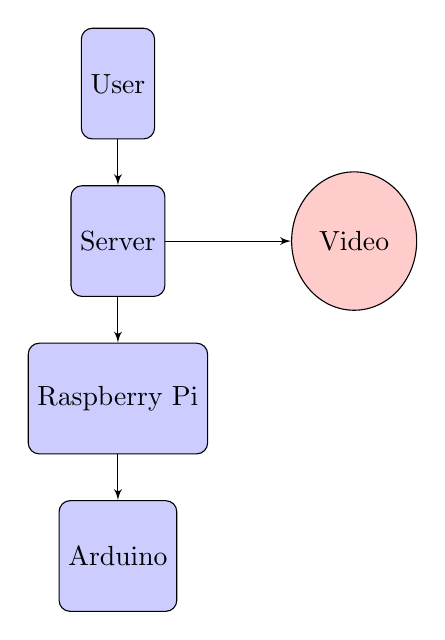
\begin{tikzpicture}[node distance = 2cm]
						% Place nodes
						\node [block] (user) {User};
						\node [block, below of=user] (site) {Server};
						\node [cloud, right of=site] (video) {Video};
						\node [block, below of=site] (pi) {Raspberry Pi};
						\node [block, below of=pi] (arduino) {Arduino};
						
						% Draw edges
						\path [line] (user) -- (site);
						\path [line] (site) -- (video);
						\path [line] (site) -- (pi);
						\path [line] (pi) -- (arduino);
						
						
					\end{tikzpicture}
				\end{center} 
				
				The reason that the user has to communicate to the Raspberry Pi through a server is because whilst roaming the Raspberry Pi will have a constantly
				changing IP address. This will make it impossible for the user to connect directly to the Raspberry Pi as the user would not know the IP address of
				the Raspberry Pi at any one time. Instead the Raspberry Pi will be constantly pinging a server with a static IP (that is, an IP which does not change).
				The user can then connect to the server and send commands to it which in turn the server will relay to the Pi, as shown in the diagram.
				
				This will allow the user and the robot to communicate to each other without them having to know each others IP address. Due to the cost of hiring a
				dedicated server, I will be hosting the server from a home computer. This shall allow me full control over the server with no additional cost added
				to the project. Because the server is only temporary I will be using the Windows 7 operating system to host it, as this is the operating system
				already installed on the computer. If the server were to become more permanent I would install an OS better suited to hosting, such as the Linux
				distribution \emph{Red Hat Linux}.
		
		\chapter{Production}
			\section{Programming}
				In order for the robot to function it must be able to carry out a specific set of instructions. Writing these instructions is called \emph{programming}.
				
				\subsection{Server}
					The first program I will write will be for the server. The main aims of this program shall be:
					\begin{enumerate}
						\item Accept incoming ping's from the robot, establish connection to the robot.
						\item Accept incoming commands from an external client. Relay these commands to the already connected robot.
					\end{enumerate}
					This will allow the user to control the robot without having physical access to the machine or knowledge of its IP address. I started off with a
					few lines of code which will echo back any incoming messages. The following code is written in the language Python 1.7.
					\lstinputlisting[language=Python, caption=serverecho.py]{examples/serverecho.py}
					I then changed this code to relay messages sent from one client (the user) to a different client (the robot) as described in the software section.
					The new code is as follows.
					\lstinputlisting[language=Python, caption=relayserver.py]{relayserver.py}
					This works by obtaining connections to both the robot and the user. The program then waits on any messages sent by the user. When a message is recived it
					overwrites the \lstinline{command} variable with the given message. Whilst it is doing this, the program constantly sends the \lstinline{command} variable to the robot,
					every 0.1 seconds, as long as the robot is currently connected to the server.
				
				\subsection{Clients}
					\subsubsection{Robot}
						I began as I did with the Server program. I created a simple program which will connect to a server, send the server a simple message and then wait to
						receive one back. Once the program has received the message it will print out the message before terminating. The program is as follows.
						\lstinputlisting[language=Python, caption=clientecho.py]{examples/clientecho.py}
						
						I then modified the program to maintain a constant connection with the server instead of terminating once it has received a messaged. I also made the
						program send the message \lstinline{user} once connected which will allow \lstinline{relayserver.py} to initiate the \lstinline{listenOnClient} thread.
						\lstinputlisting[language=Python, caption=clientconnect.py]{examples/clientconnect.py}	
						
						The output of running \lstinline{clientconnect.py}\  directly after running \lstinline{clientconnect.py}\ is shown below.
						\lstinputlisting[caption=echolog.txt]{examples/echolog.txt}
						
						However the robot needs to identify itself as \lstinline{robot} instead of \lstinline{user}. This is simply changed by replacing \lstinline{s.send('user')}
						with \lstinline{s.send('robot')}. And because the robot only receives commands and does not give them, sending constant updates as shown
						\lstinline{clientconnect.py} is pointless. Instead it would be much better to only receive messages and then act upon them. I revised the code to
						implement these changes. \lstinputlisting[language=Python, caption=robotconnect.py]{examples/robotconnect.py}	
						
						The program now needs to connect to the Arduino and pass on the given messages so that the Arduino can control the motors which in turn move the robot. In
						order to do this I will need to use programming library, or modules as they are called in Python. A library is a set of code which allows the programmer to
						easily accomplish something which would have taken a long time otherwise. A suitable analogy would be that cooking recipes do not list the instructions that
						the chef would need to carry out in order to make flour. The flour is already made and the chef does not need to know how flour is made or what it is
						composed of. A programming library is an already made piece of code which simplifies the development of the rest of the program.
						
						Most programs contain a set of standard a libraries which are included by default. However it would be impossible to include enough libraries that would cover every
						possible situation. Instead the developers of the language decide upon which features would be most commonly needed and then design libraries in order to provide
						those features. Since communicating between the Pi and the Arduino via USB serial is a substandard case, a library to do such a thing is not included in Python's
						standard libraries. Instead I will use a user made library to accomplish this task. My library of choice is PySerial\cite{pyserial}.
						
						In order to run the following program the computers Python instillation must have the PySerial library installed. This is done simply on
						the Raspberry Pi by typing the following command in the terminal \lstinline{pip install PySerial}. The process should be the same on all
						Linux based operating systems with Python 2.7 installed. PySerial allows for messages to be sent via USB Serial. I'm using this to send
						the messages that Raspberry Pi receives to the Arduino. I made this simple program which will receive incoming messages from the relay
						server and send them over the USB cable by using PySerial.
						\lstinputlisting[language=Python, caption="piclient.py"]{piclient.py}
						
						I deigned the client in such a manner that if it fails to connect to the server it will try again and again as long as the program is running
						This is useful as most of the time I will not have physical accesses to the Raspberry Pi, so I need to insure that the program remains running.
						I accomplished this continuous running through the use Exceptions. By using exceptions one can "catch" an error and then tell the program to
						something special in regard to this error. In this case when the client failed to connect or it disconnected it threw a
						\lstinline{connection failed} error. Normally this would result in the program crashing, but because the program now catches any errors the program
						continues running after closing any opened sockets. Because the connecting code in contained within the \lstinline{while True:} block the program will
						attempt to connect again after reviving the disconnection error.
						
						The messages sent to the Arduino are in the format listed in key.txt
						\lstinputlisting[caption="key.txt"]{examples/key.txt}
						
						So if I wanted to move the first motor forwards at maximum power I would send a message to the Arduino saying "f 1 255".
						
						In order to move the motors using the Arduino I used the Adafruit motor shield\footnote{\url{http://www.adafruit.com/products/81}} and the
						accompanying library\footnote{\url{https://github.com/adafruit/Adafruit-Motor-Shield-library}}. In order interpret the commands as listed
						above I used the example made by Mushfiq Sarker\cite{serialread}.
						\lstinputlisting[caption="arduinoserial.ino", language=C]{arduinoserial/arduinoserial.ino}
						
						This program will receive messages from the Raspberry Pi running the \lstinline{piclient.py} script and then move the motors in accordance
						with the message sent as detailed in \lstinline{key.txt}. This is the last program which will run on the Raspberry Pi and it is absolutely
						critical that it runs without fault as the embedded nature of the platform will make it very difficult to change without physical accsess
						to the robot.

					\subsubsection{User}
						The user will connect to the server through a website. The website will use websockets to connect to the server. Websockets are a
						relatively new protocol. They are part of the JavaScript programming language and enable client side communication over the internet.
						In order for the user to use the website it must have a GUI, a graphical user interface. This is done through the use of HTML and 
						CSS. Because my HTML/CSS skills are lacking somewhat I opted to use the interface designed by Andy Harris\cite{dummies}.
						But with some adjustments to accommodate for the messaging the relay sever and thus robot with the right commands.
						\lstinputlisting[caption=usersite.html,firstline=45, lastline=139]{usersite.html}
						
						I omitted the CSS code and chose only to display the logic code in the example in order to conserve space. The full html file
						can be found at \lstinline{usersite.html} with CSS intact.
						
						The above code connects to the relay server when the user presses the \lstinline{connect} button. Upon a successful connection
						the client identifies itself as a user in the \lstinline{onOpen} function. Once connected the client checks to see if any arrow
						keys have been pressed every 100 milliseconds. If they have it sends the appropriate command to relay server. This enables the
						user to control the robot through use of the arrow keys on their keyboard. This may need to be updated in the near future to
						accommodate for mobile devices who do not have a physical keyboard. It also allows the user to send commands manually via the
						text box below the output field. The arrow keys however significantly increase the speed at which the user may react. Typing in
						command manually will enable the user to have very precise control over the robot. If the user fails to press any key the client
						will send the message to indicate the robot should move no motors. This still allows the robot to coast if it was moving before,
						but will prevent it from veering off uncontrollably if it loses connection from the relay server.
						
						If I wish for the response time between the user pressing the arrow keys and the robot responding to be shorter, I could change the
						function \lstinline{loop} to run at shorter intervals than every 100 milliseconds.
					
					\subsection{Connecting}
						After testing \lstinline{relayserver.py} with \lstinline{usersite.html} a problem soon became evident, the protocol which websockets
						uses and the raw TCP protocol which \lstinline{relayserver.py} uses are not initially compatible. After further research I found
						a website\cite{websockets} which explains the differences between the two and offers a possible solution. However after many
						attempts I could not replicate  Yang Zhang's method successfully. Instead I opted for the Tornado library which promised to make
						the connecting to WebSockets a lot quicker and cleaner than my previous attempts. I wrote a simple server application which
						will echo any received messages. This was based on the echo test provided by the Tornado documentation\footnote{\url{http://www.tornadoweb.org/en/stable/}}
						\lstinputlisting[language=Python, caption=websocketserver.py]{examples/websocketserver.py}	
						
						I used WebSocket echo test website\footnote{\url{http://www.websocket.org/echo.html}} in order to test whether the server was working.
						Initially there was no response on either side, but after an hour of debugging I found out that is was the function call
						\lstinline{tornado.web.Application([(r"/ws", WSHandler)])} causing the problem, particularly the \lstinline{"/ws"} string.
						The \lstinline{"/ws"} string made it so that in order to successfully connect to the server you have to add \lstinline{"/ws"} to the
						end of the address. After changing \lstinline{ws://derekbot.servegame.com:25565} to \lstinline{ws://derekbot.servegame.com:25565\ws}
						everything worked perfectly.
						
						After determining the success of the echo test, I then implemented it into the original \lstinline{relayserver.py}. The updated changes
						have been saved as \lstinline{relayserverfinal.py}. I also implemented the error catching as seen \lstinline{piclient.py} and for the same
						reasons as listed before.
						
						\lstinputlisting[language=Python, caption=relayserverfinal.py]{relayserverfinal.py}
						

						After further testing I discovered that the sending of two messages close to one another by \lstinline{relayserver.py} caused a backlog
						to be built up in \lstinline{piclient.py}. It also caused the second motor to stop working seemingly at random. After many hours of
						testing I was still unable to determine the origin of this problem. Instead I decided to modify \lstinline{usersite.html} to send a
						single message for each movement command in the form of \lstinline{forwards, backwards, right, left}. Once received
						\lstinline{piclient.py} will translate those messages into the format which was used earlier (\lstinline{x y zzz}) and send them
						over serial to the Arduino. I also added a short delay in \lstinline{piclient.py} between sending the messages as an extra precaution.
						The changes are shown below, with the original code being omitted for reasons concerning the size of this report.
						
						\lstinputlisting[language=Python, caption=piclient.py, firstline=12, lastline=39]{examples/piclient2.py}
						\lstinline{...}
						\lstinputlisting[language=Python, firstline=62, lastline=69]{examples/piclient2.py}
						
						This works be defining 4 functions, \lstinline{forwards}, \lstinline{backwards}, \lstinline{right} and \lstinline{left}. Each function
						sends the necessary strings over the serial connection to the Arduino which will accomplish the movement desired. When
						\lstinline{piclient.py} receives a string it attempts to run the function which has the name of the received string. In most cases this
						would be one of the movement words sent by \lstinline{usersite.html}, which would work fine. But if for some reason this is not the case
						I used error catching to insure that the program continues to run smoothly.
						
						After testing the applied changes I noticed that the connection no longer dropped for no apparent reason, and that both motors were
						fully operational, and responded to the user input quickly and accurately.
						
						I then loaded the program \lstinline{piclient.py} onto the Raspberry Pi. To do this I had to connect to the Raspberry Pi over SSH, it is
						possible to do this on windows by using using a program called Bitvise or PuTTY, whilst if you are running a Linux operating system, there
						is SSH included by default. This can be accessed by the command \lstinline{ssh user@ip}.
						
						\begin{figure}[h]
							\caption{Connecting to a Raspberry Pi via SSH on windows.}
							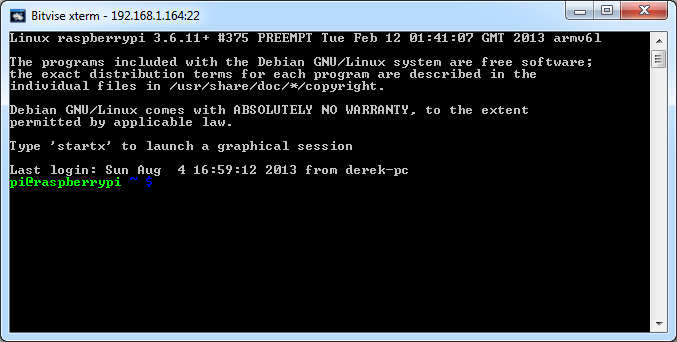
\includegraphics[width=\textwidth,height=\textheight,keepaspectratio]{images/ssh}
						\end{figure}
						
						Once connected I copied over the files and ran \lstinline{piclient.py} on the Raspberry Pi. However I found that the commands written to
						the Arduino became slower and slower as time went on, resulting in massive delays. This was easily fixed however by "flushing" the input
						and output buffers, essentially clearing them and prevent any backlog from building up in them. To do this I employed 3 functions which
						were part of the \lstinline{serial} object in the \lstinline{pyserial} library. The functions were added at the end of the
						\lstinline{while True} loop after all the serial writing had taken place. The amended code is as follows.
						
						\lstinputlisting[language=Python, caption=piclient.py, firstline=66, lastline=73]{examples/piclient3.py}
						
						I tested this amendment thoroughly and found that it prevent the large delay that I was experiencing beforehand, increasing the stability
						of the program and the robot as a whole massively.
						
					\subsection{Assembly}
				The first component assembled was the chassis. The chassis are in the form of a 110x85x70mm 3mm acrylic box. Each side of the box was first
				designed in the computer program called 2D Design\footnote{\url{http://www.techsoft.co.uk/products/software/2D_Design_V2.asp}}. 
					
				The design was then printed onto a laser printer. The laser printer cut out the designs to a degree of accuracy that is impossible for any							human hand.		
						
				The box was then assembled using a type of glue called Acrylic Cement. Special care was taken to align the sides of the box, but due to the thinness
				of the acrylic (only 3mm) perfect aligning on the box was not accomplished. However this is only a minor detail and it is easily overlooked.
						
						\begin{figure}[h]
							\caption{The acrylic box partially assembled.}
							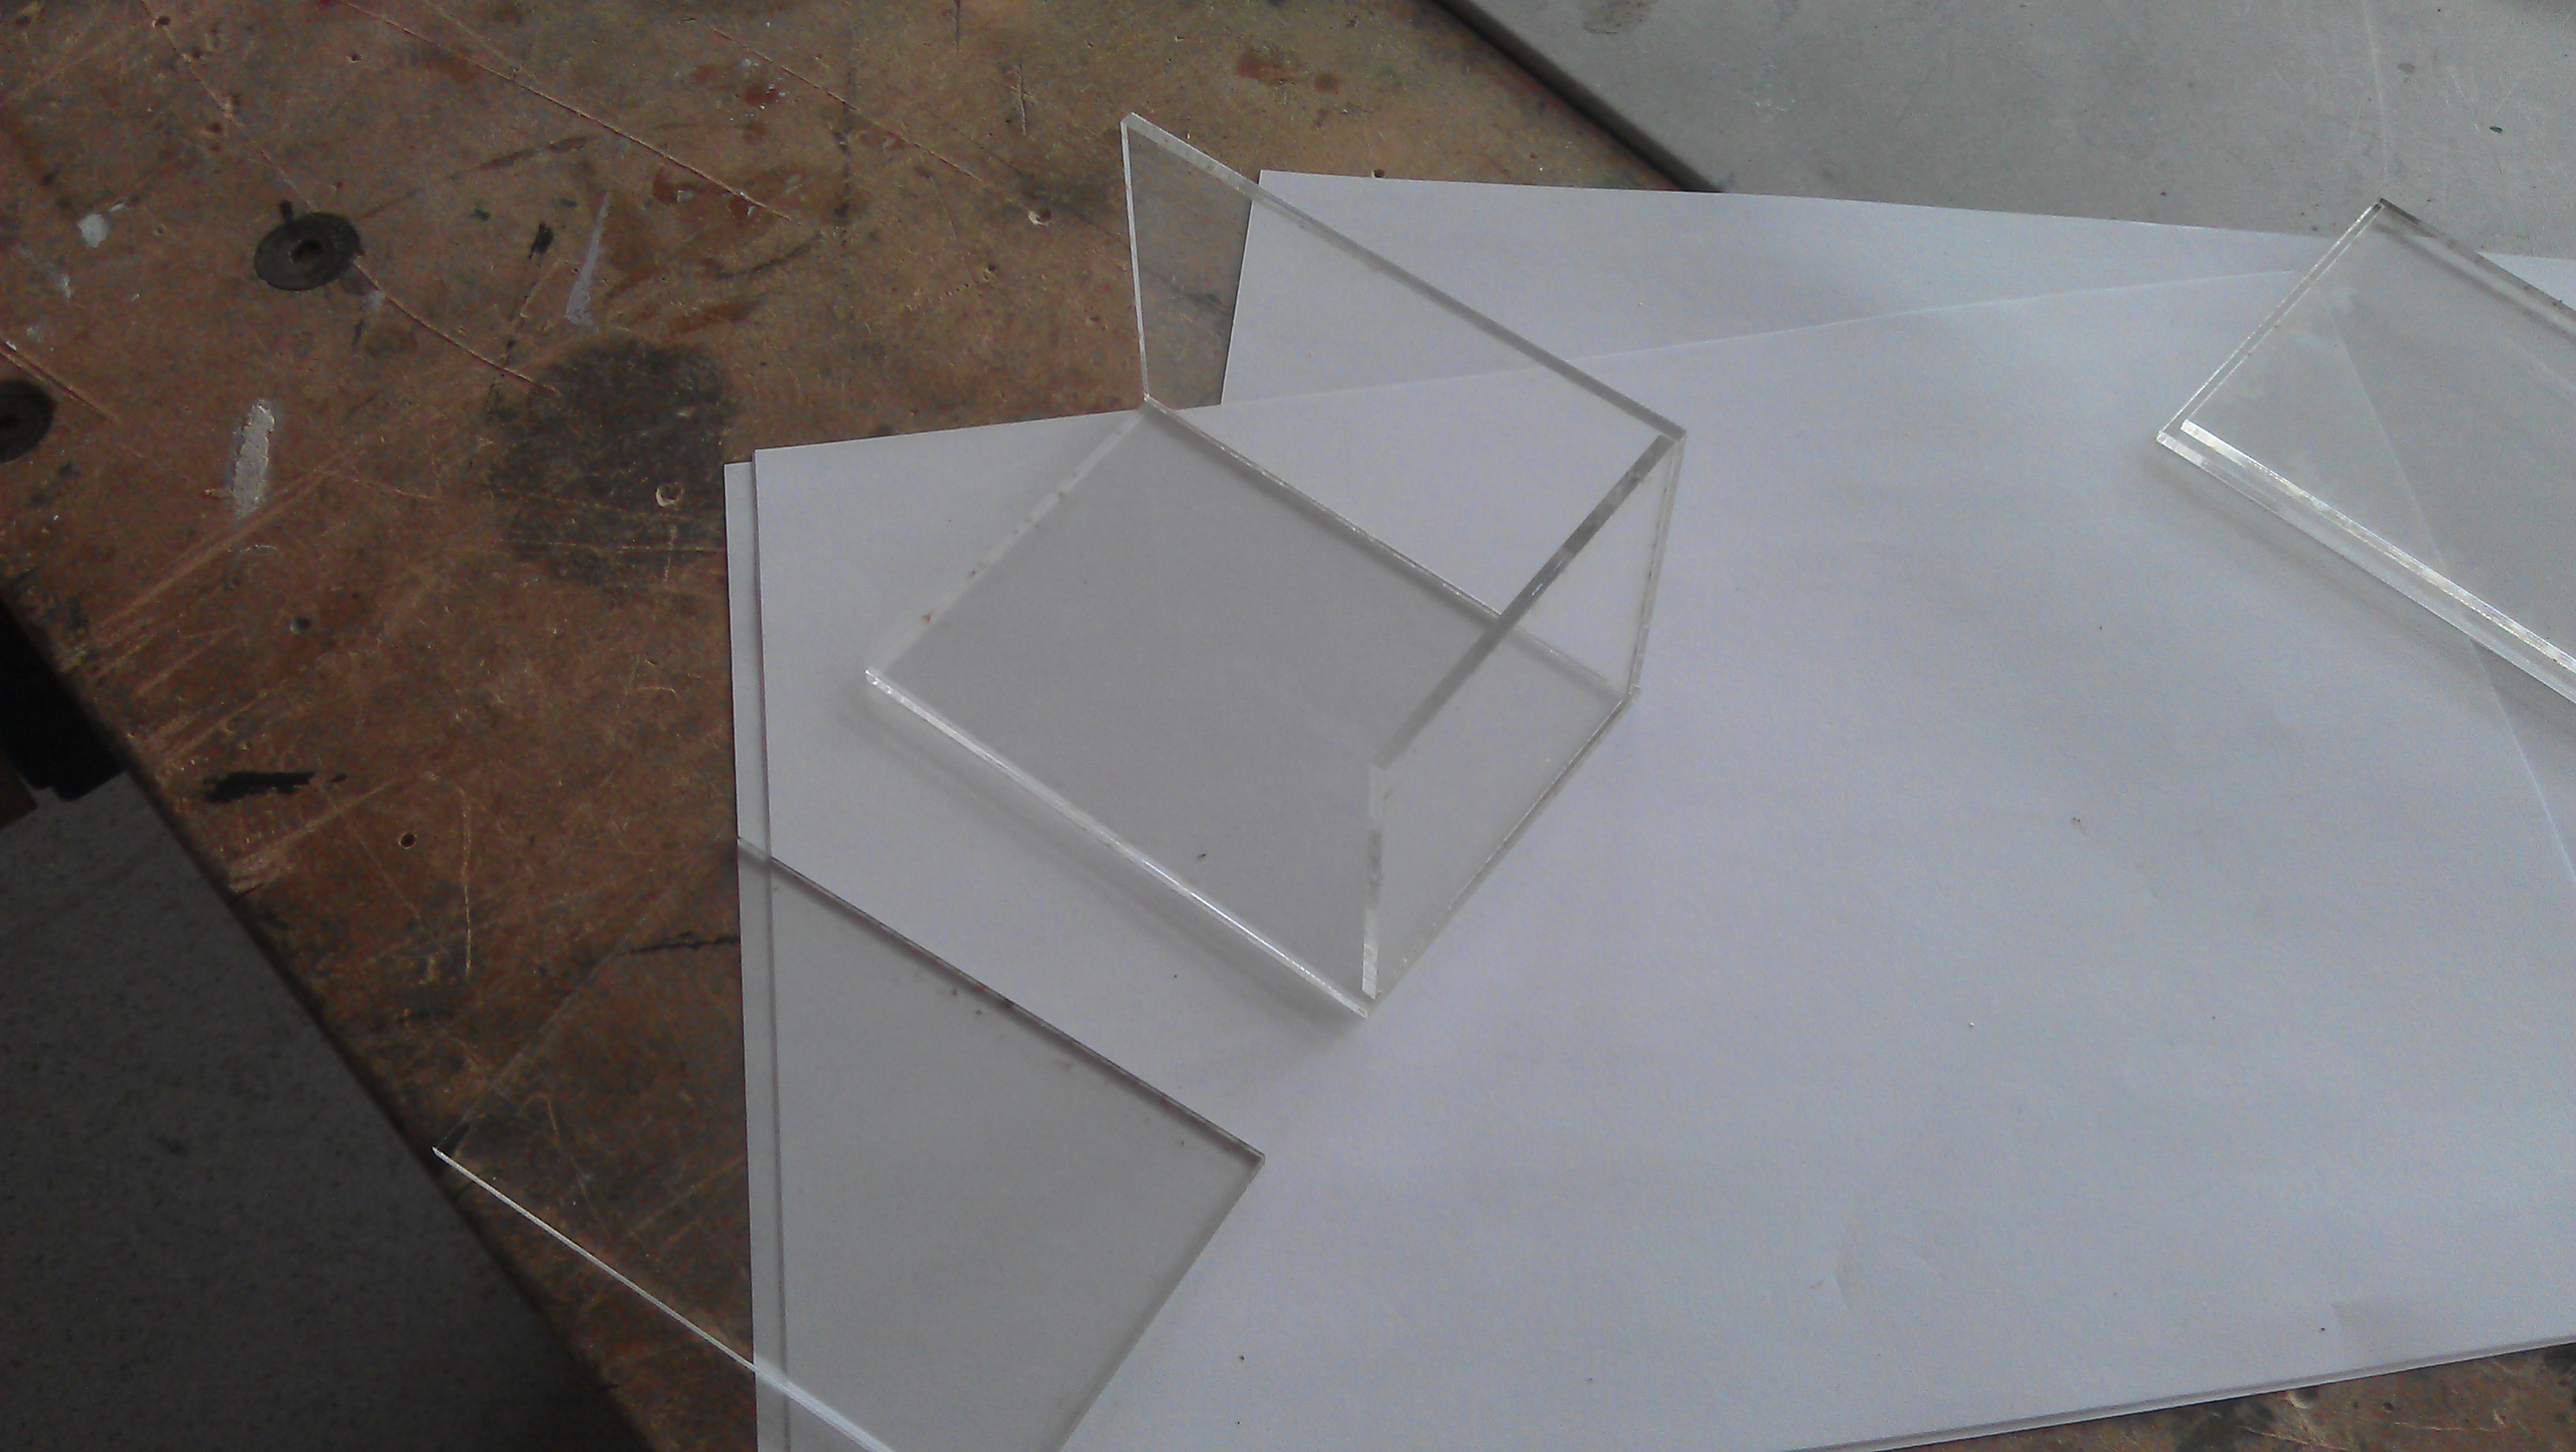
\includegraphics[width=\textwidth,height=\textheight,keepaspectratio]{images/almostdone}
						\end{figure}
						
						I then had to drill the wormdrive gear boxes to the chassis. Unfortunately during the drilling a minor crack formed around the edges of one of the holes.
						I did not fully tighten the nut and bolt around this hole in a somewhat hopeful attempt to prevent the crack from spreading any further.
						
						\begin{figure}[h]
							\caption{Holes in the box being drilled.}
							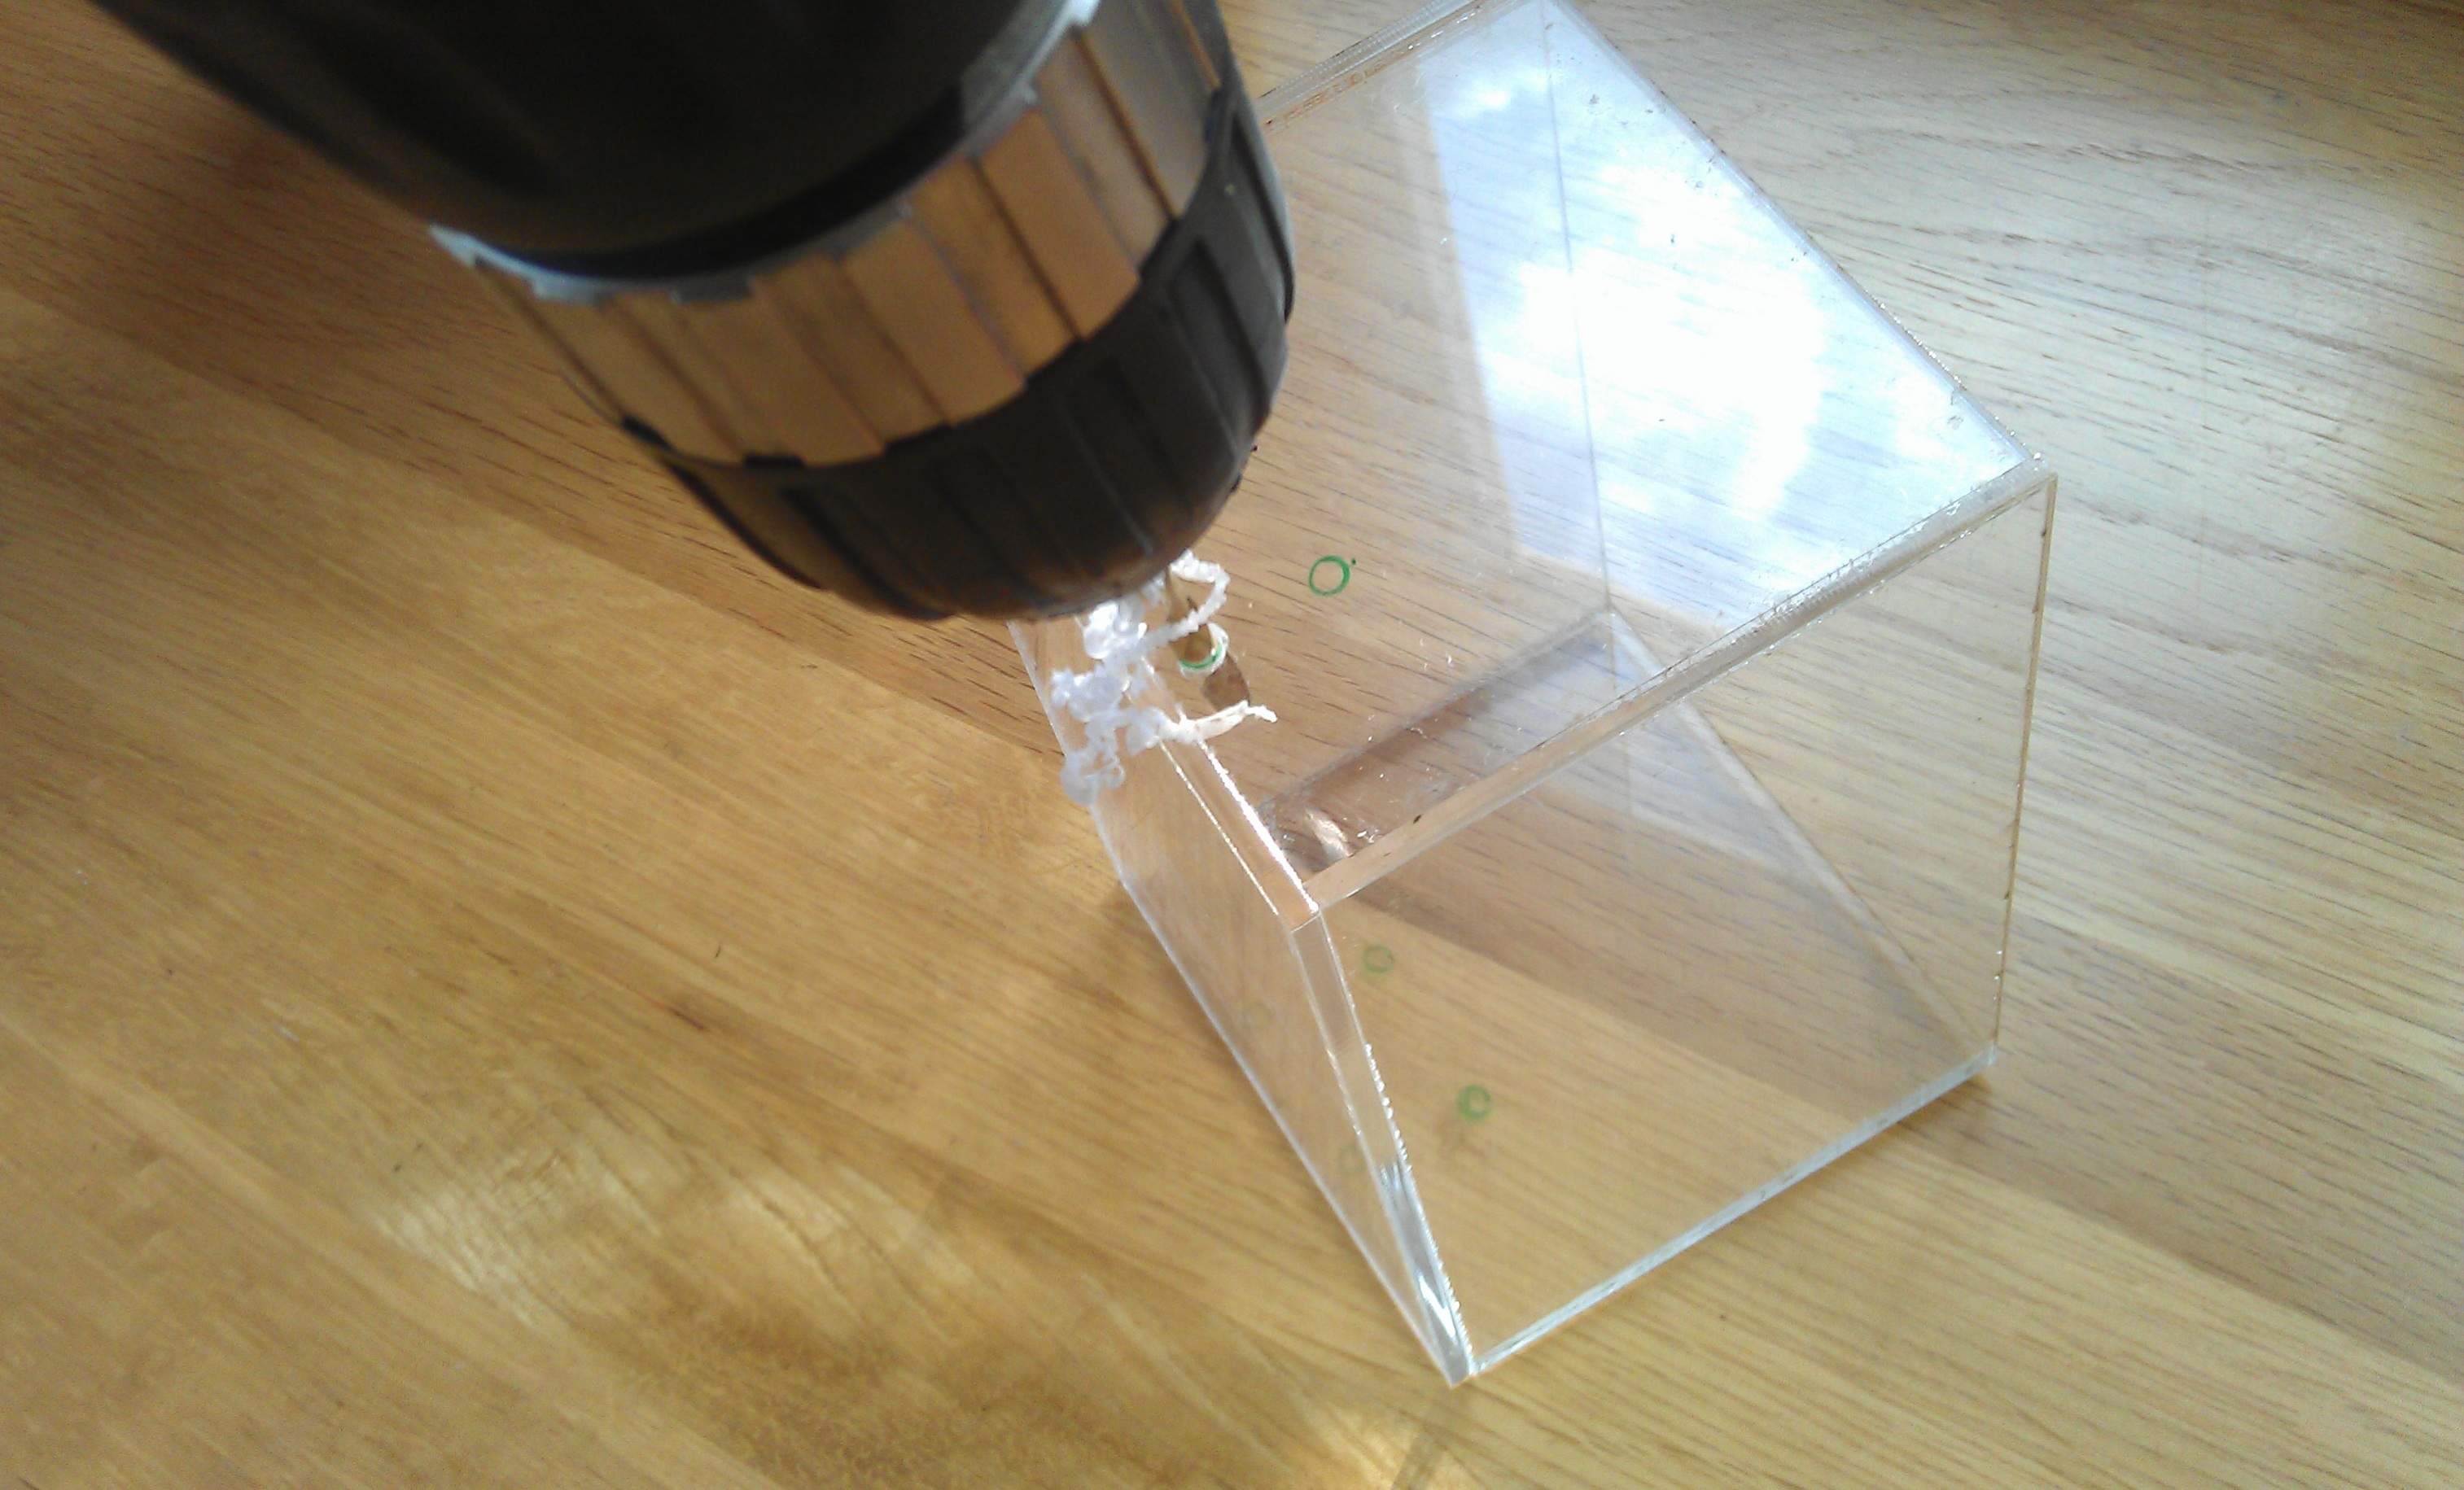
\includegraphics[width=\textwidth,height=\textheight,keepaspectratio]{images/drilldrilldrill}
						\end{figure}
						
						After drilling the holes into the box I attached the wormdrive gear motors and the accompanying wheels, axis and tracks. I noticed that the tracks were
						a little tight, possibly a symptom of making the box a little bit to long. But at this point there was little to be done about that.
						
						\begin{figure}[h]
							\caption{Robot with assembled chassis and tracks.}
							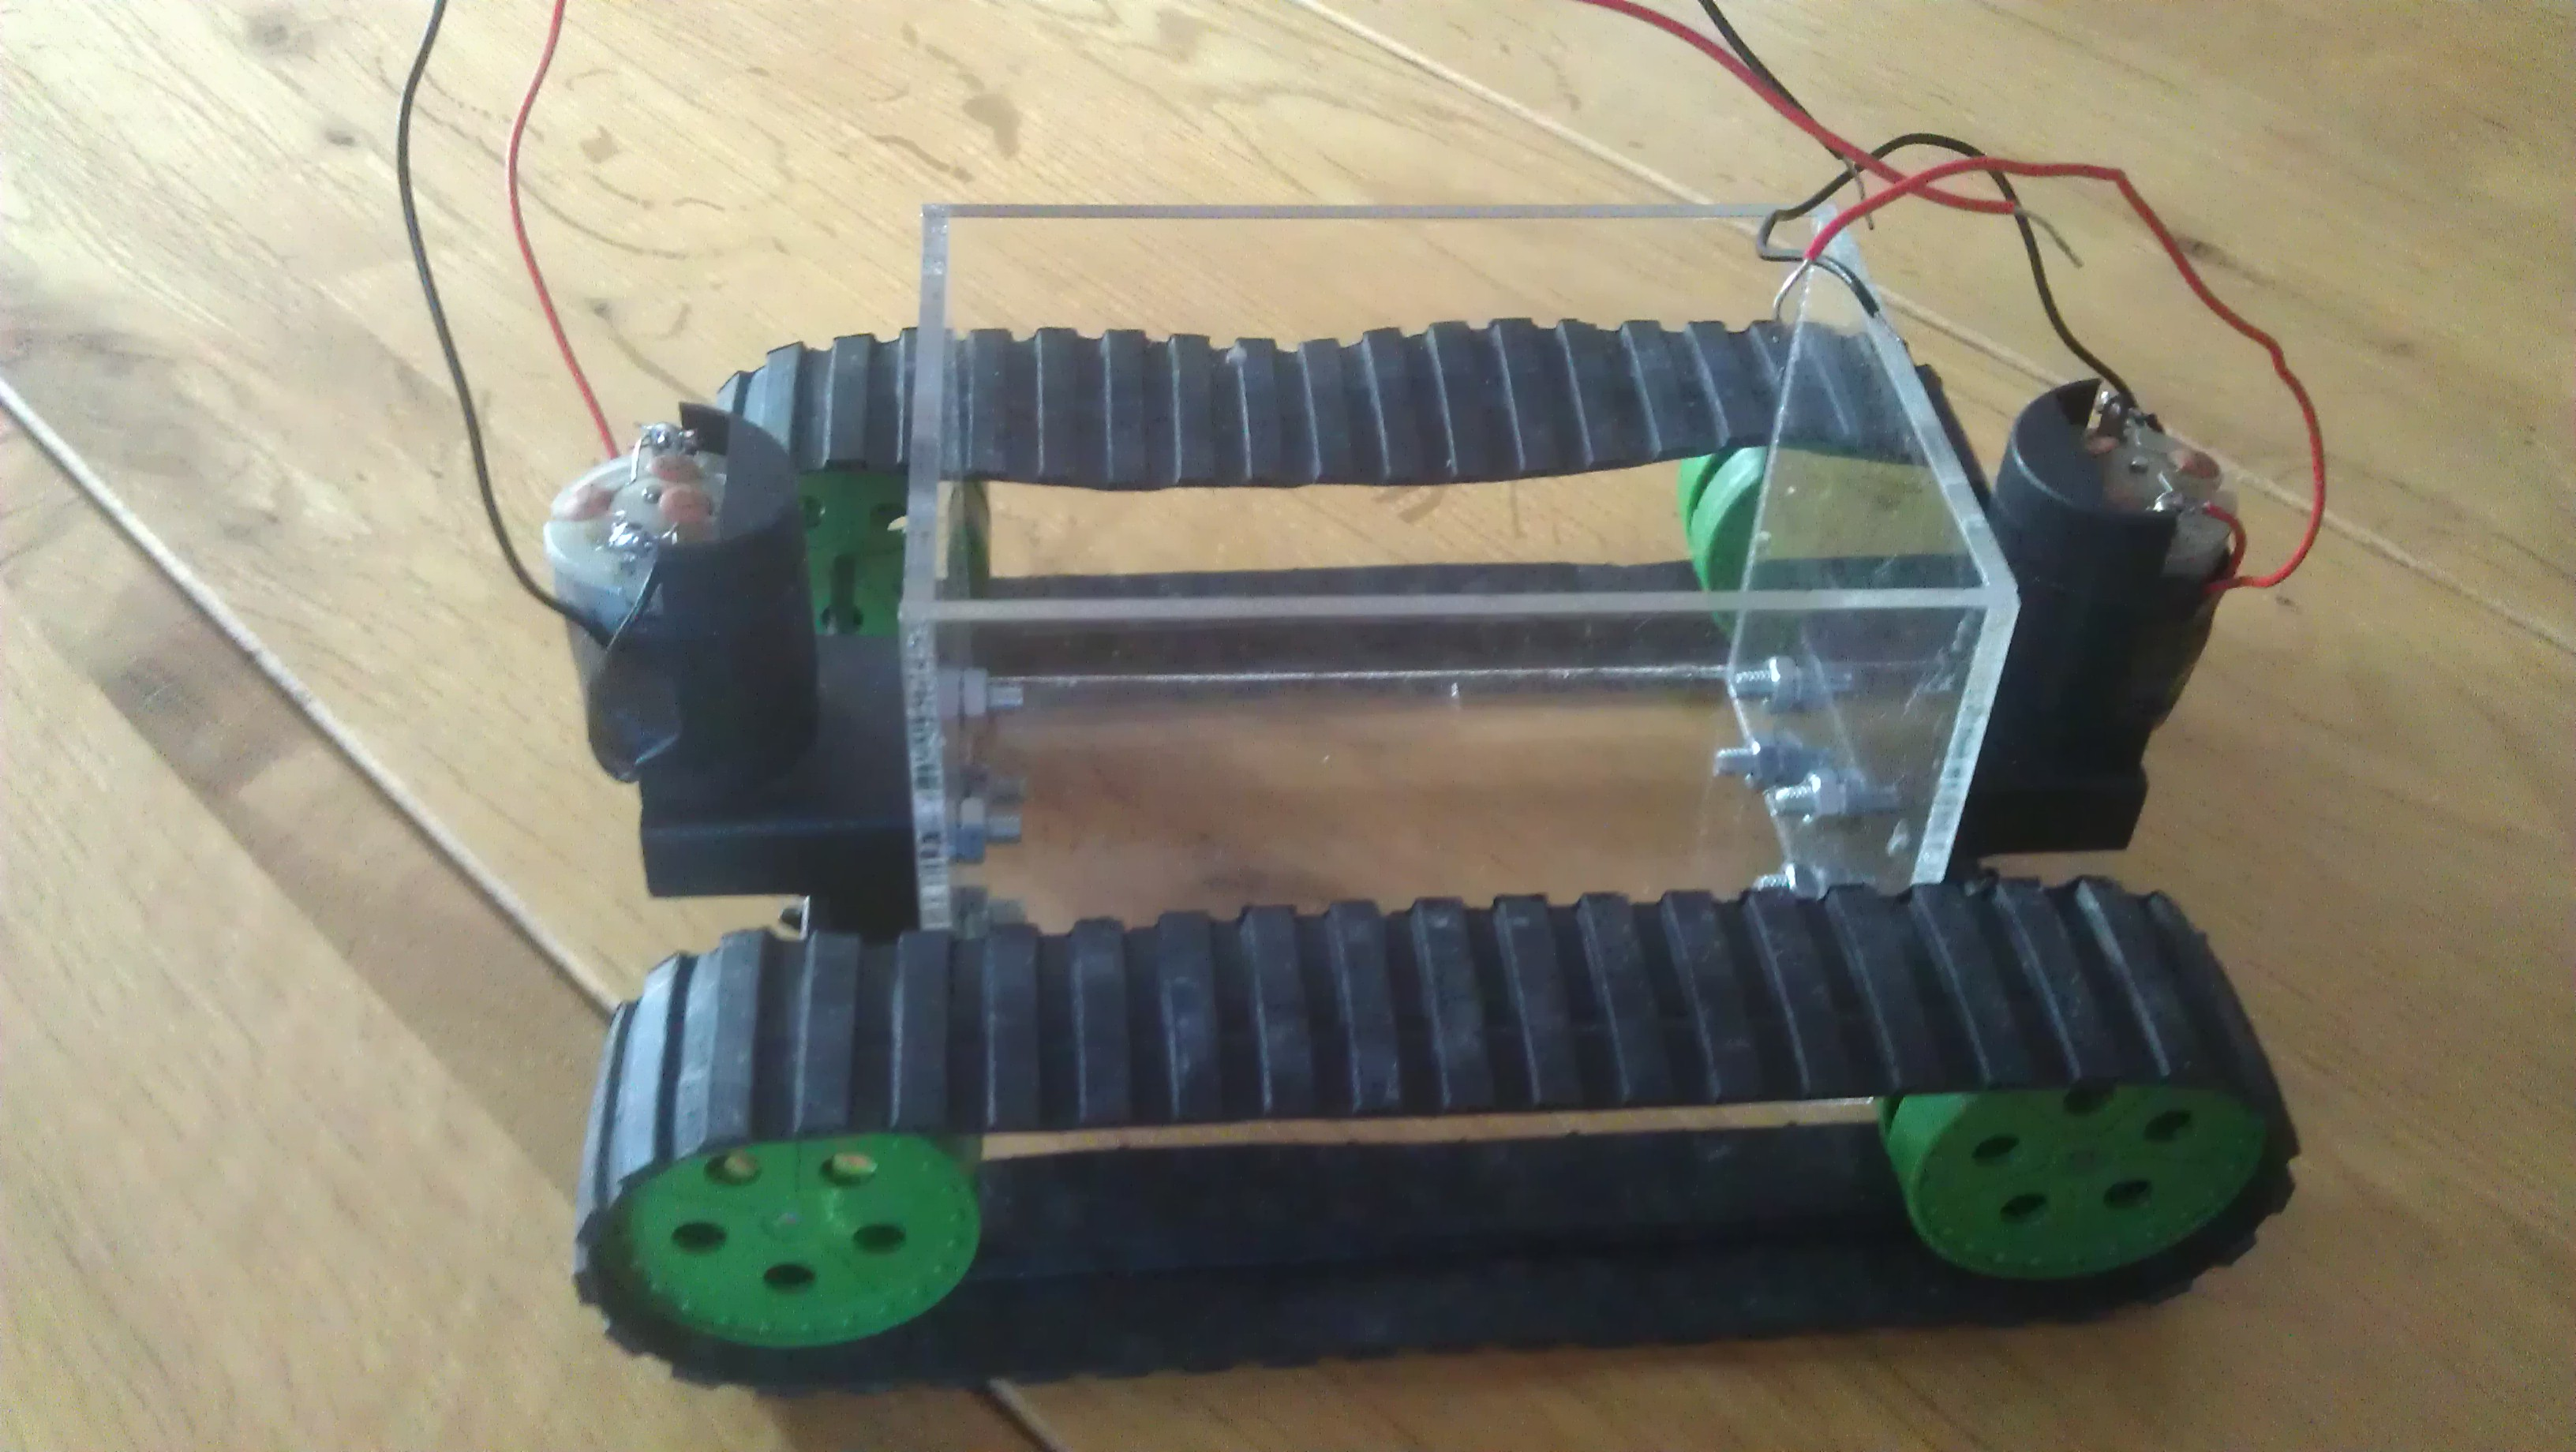
\includegraphics[width=\textwidth,height=\textheight,keepaspectratio]{images/noinsides}
						\end{figure}
						
						I then places the components inside the chassis, using bubble wrap for scratch protection. I was a little concerned about the use of bubble wrap, as it may
						cause the components inside the box to overheat. I may have to change the method of protection at a later date if this becomes a problem.
						
						\begin{figure}[h]
							\caption{Assembled robot}
							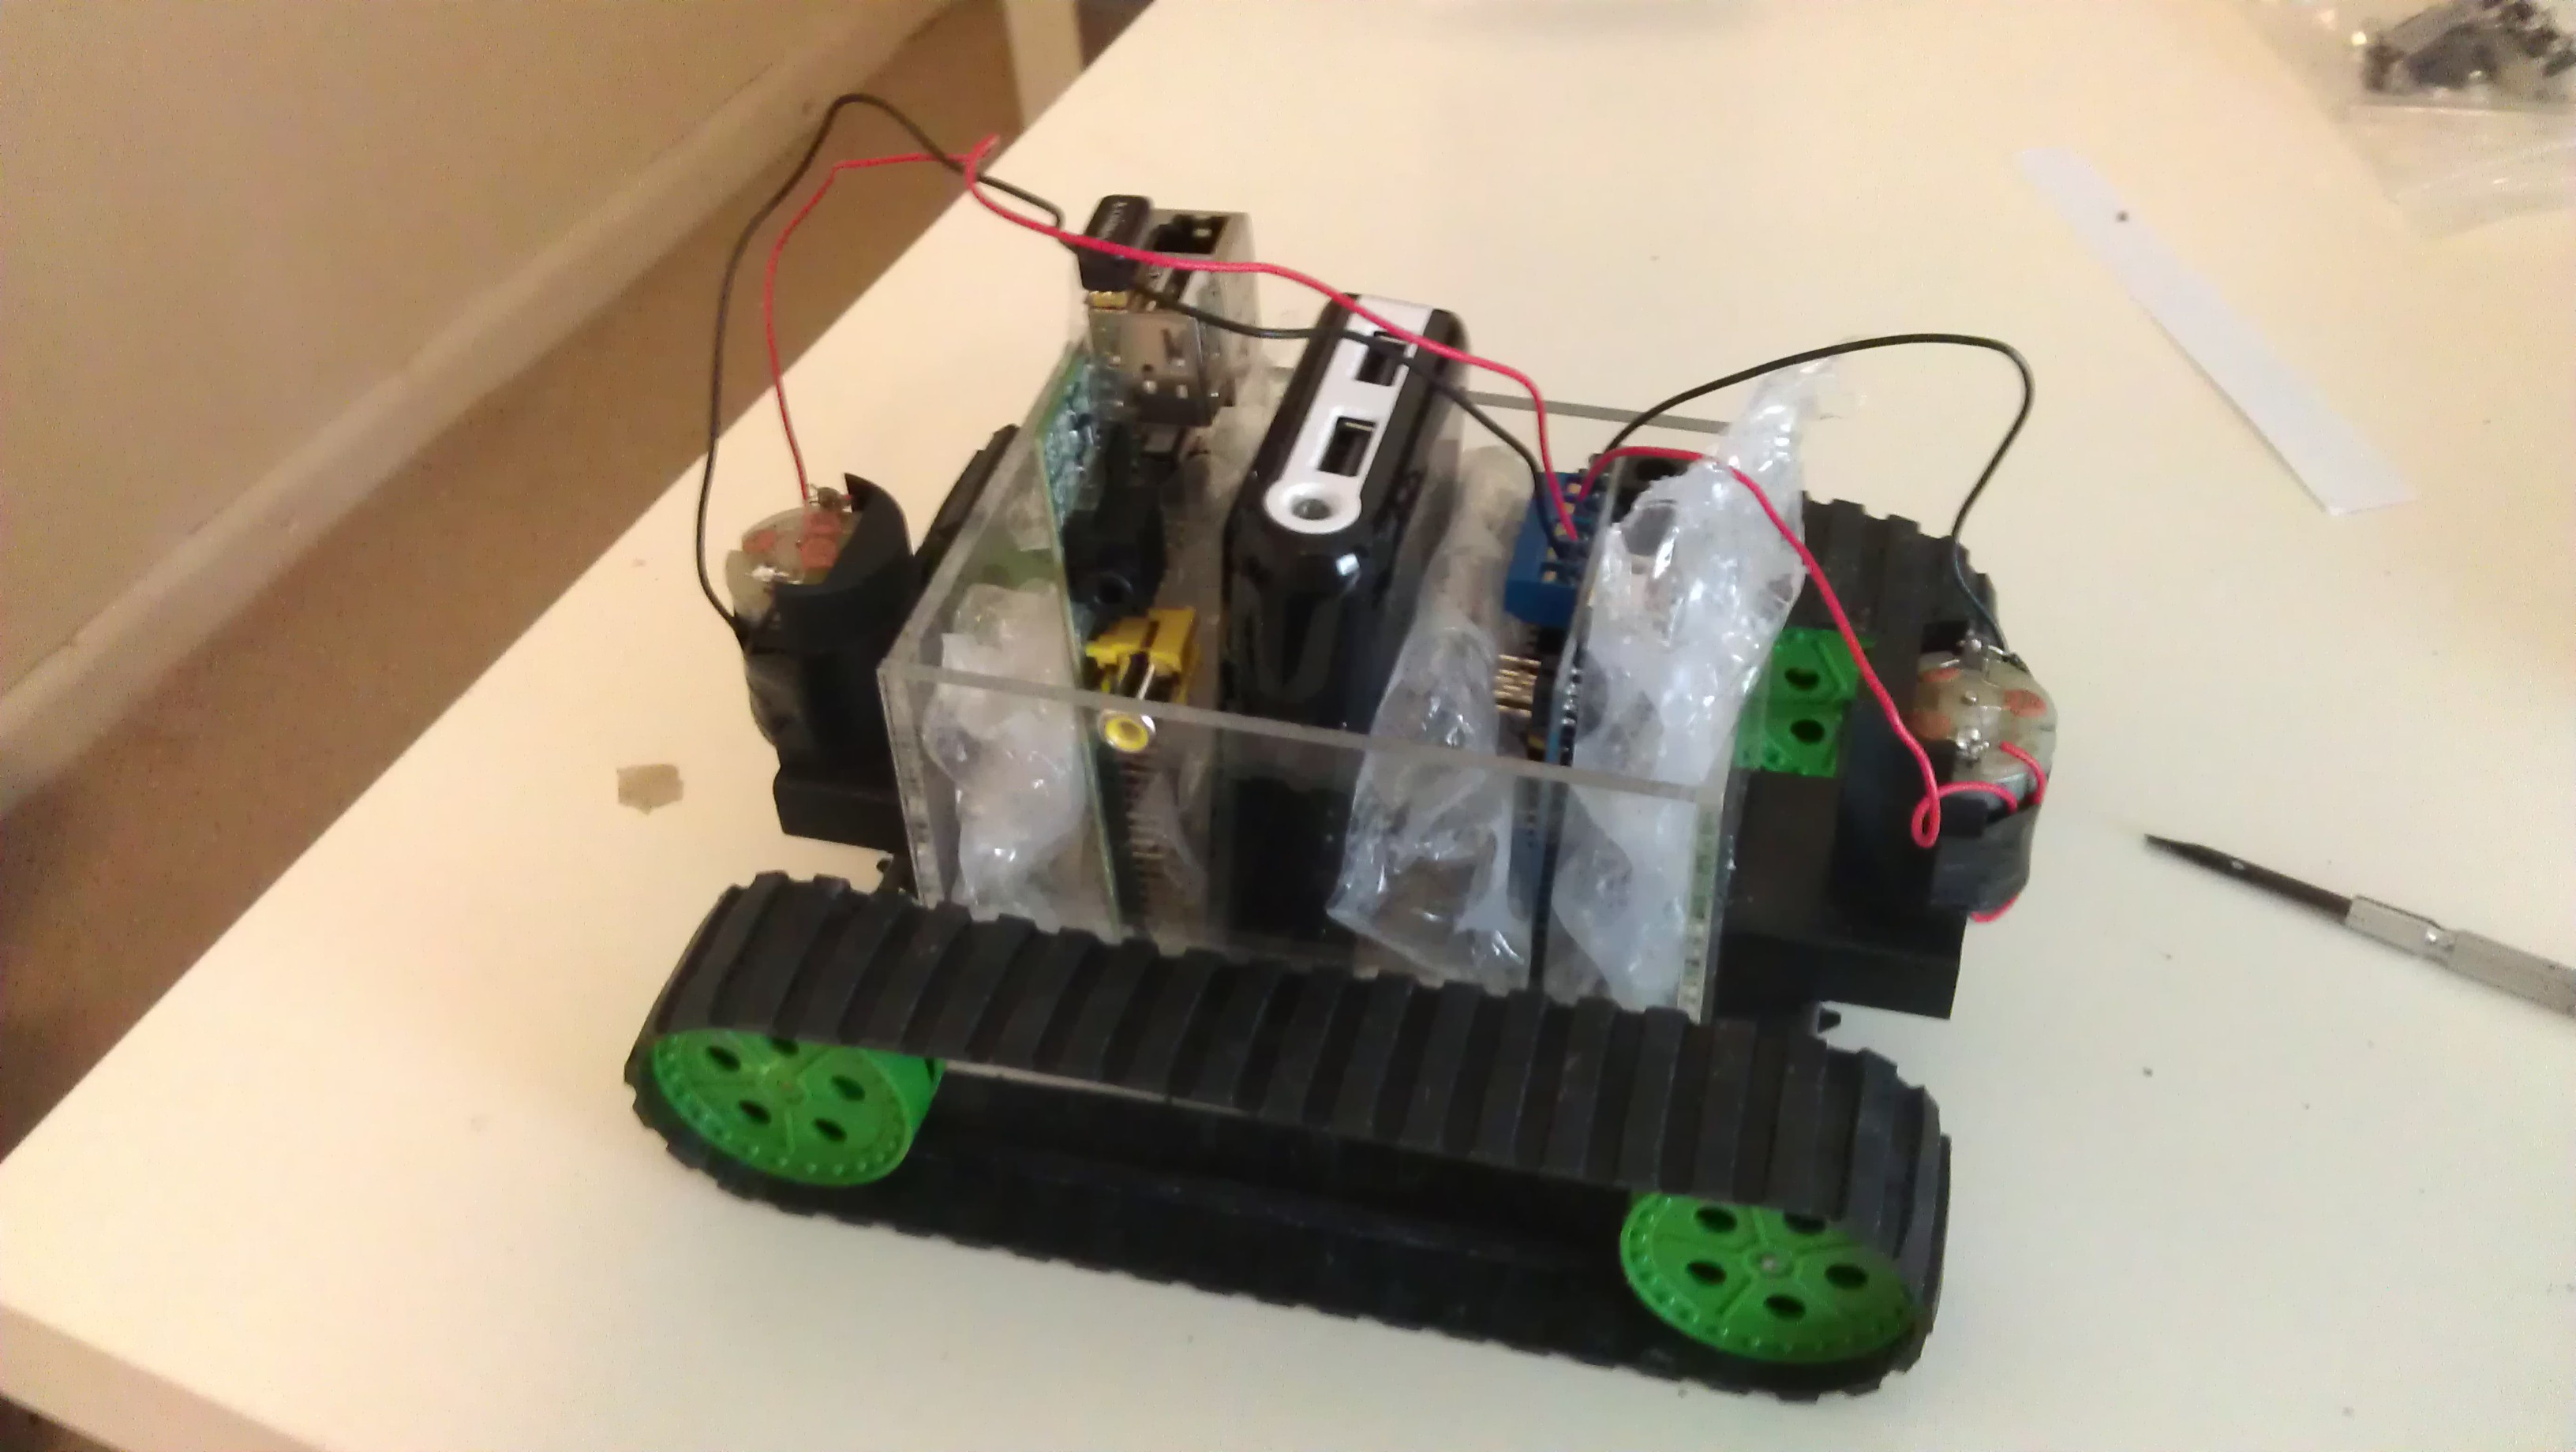
\includegraphics[width=\textwidth,height=\textheight,keepaspectratio]{images/nowires}
						\end{figure}
						
						In order to get the robot to turn each track has to be controlled by an individual motor. My setup as shown above did not allow that as
						each motor controlled both tracks, limiting the robots movement to only backwards or forwards. If the motors were to turn in different
						directions it would cause the wheels to spin in their tracks, resulting in a net movement of zero. If only one of the robots motors were to turn it
						force the worm drive gear of the non-turning motor to move, sawing away at the gear and permanently damaging it. To fix this I had to
						drill a hole in two sets of wheels on opposite sides and ends to the robot. The holes were wider than the axle itself causing the motor
						connected to the axle to have no direct connection to that wheel itself and thus leaving it unable to influence or be influenced by that
						side of the motor. This essentially limits each motor to only one side of the robot. By making the motors move in opposite directions it
						is now possible to turn the robot. Please see figures ~\ref{fig:schem1} and ~\ref{fig:schem2} for further explanation.
						
						\begin{figure}[h]
							\caption{Schematic showing the effect of drilling holes in the wheels. \cite{roverschem}}
							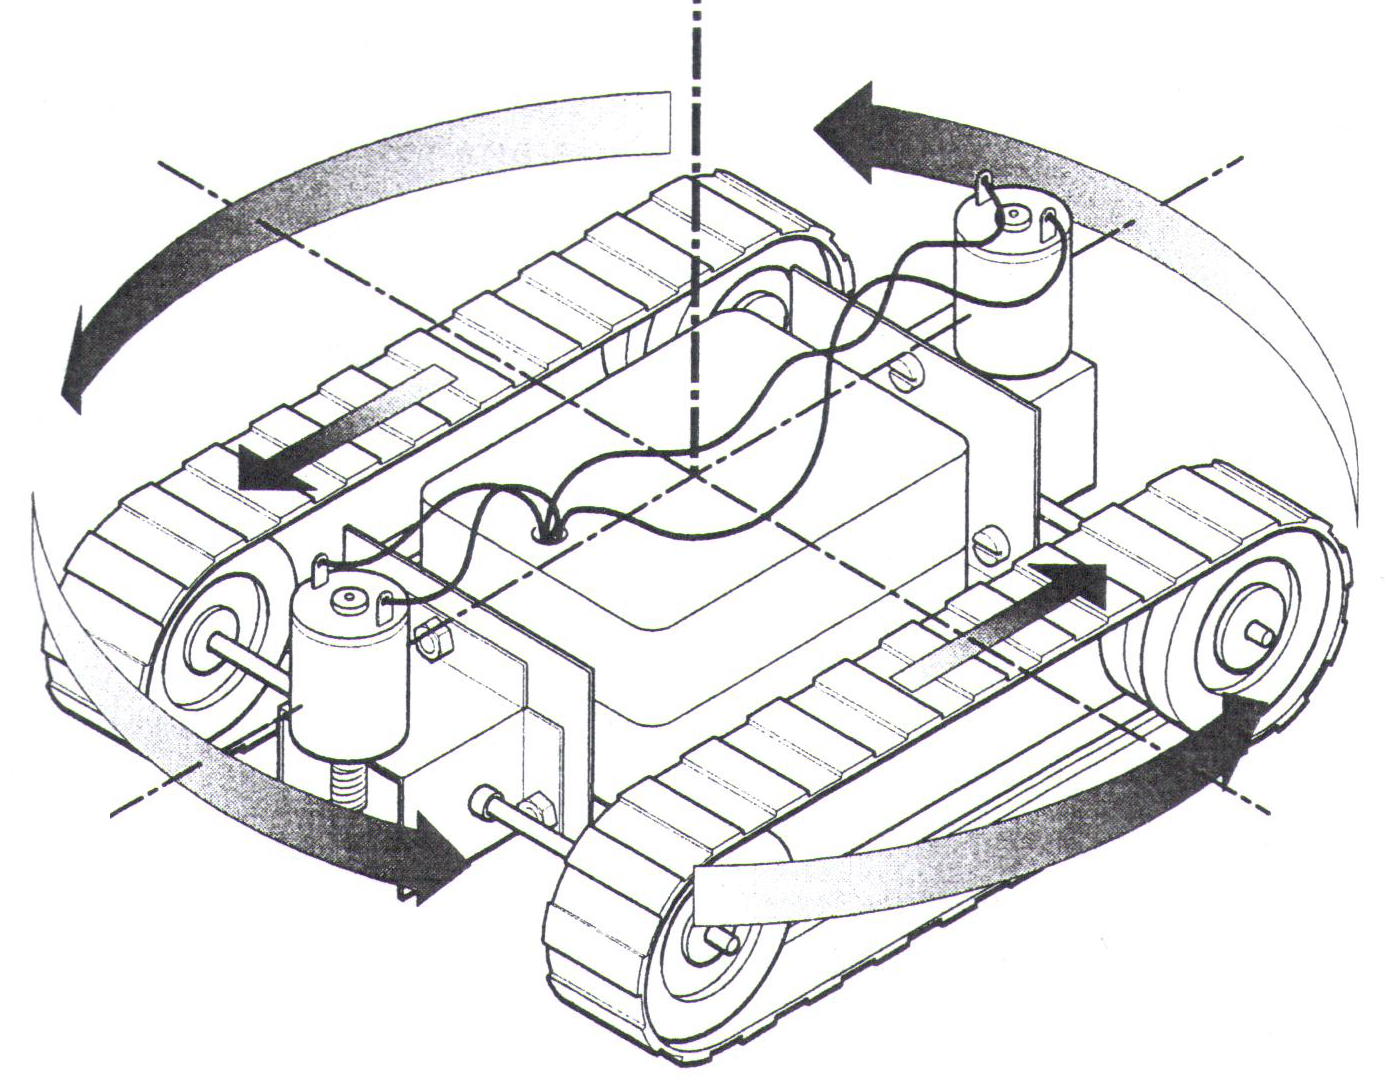
\includegraphics[width=\textwidth, height=\textheight, keepaspectratio]{images/scem1}
							\label{fig:schem1}
						\end{figure}
						
						\begin{figure}[h]
							\caption{Schematic showing which wheels need to be loose and which need to be fixed so that the robot can turn.\cite{roverschem}}
							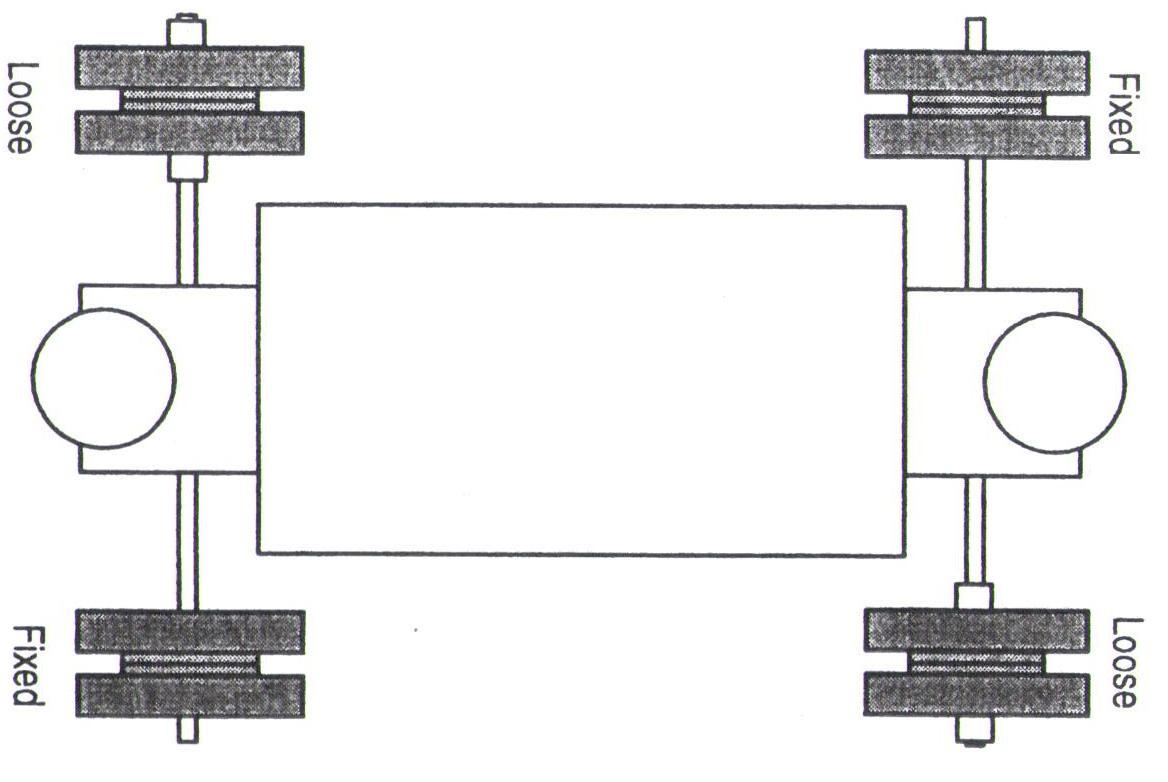
\includegraphics[width=\textwidth,height=\textheight,keepaspectratio]{images/scem2}
							\label{fig:schem2}
						\end{figure}

						With this final alteration the robot is now essentially complete, it can be driven from a web enabled device as a home pc as
						long as the robot is also connected to the internet and \lstinline{relayserverfinal} is runnning. 
	\begin{thebiblio graphy}{9}
			\bibitem{raspclock} Raspberry Pi Config on Github (May 2013). Retrieved from \url{https://github.com/asb/raspi-config/blob/master/raspi-config}.
			\bibitem{robotdef} The Oxford Compact English Dictionary (1996). Definition of \emph{robot}.
			\bibitem{rasporder} Elinux.org, May 2012. Raspberry Pi Buying Guide.
			\bibitem{pyserial} Chris Liechti (2010). pySerial's documentation. Retrieved from \url{http://www.wikibooks.org}.
			\bibitem{websockets} Yang Zhang (Dec 18, 2009). Web Sockets tutorial with simple Python server.
			Retrieved from \url{http://yz.mit.edu/wp/web-sockets-tutorial-with-simple-python-server/}
			\bibitem{serialread} Mushfiq Sarker (June 5th, 2012). Reading Serial Input with Commands and Numbers. Retrieved from
			\url{http://www.inventige.com/arduino-reading-serial-input-with-commands-and-numbers/}.
			\bibitem{roverschem} Middlesex University. Magic of engineering rover booklet. Supplied with kit purchased from
			\url{http://www.mindsetsonline.co.uk/product_info.php?products_id=699}
	\end{thebibliography}
                      
        


\end{document}
